\section{Introduction}
\SectionPage

% \subsection{Data analysis}
\begin{frame}
    \frametitle{Data analysis}
    \vspace*{\fill}

    \begin{columns}[onlytextwidth, c]
        % Column 1
        \begin{column}{0.495\textwidth}
            \begin{itemize}[<+-|alert@+>]
                % \item Process of \structure{breaking down} a whole into its constituent parts for closer evaluation.
                \item Breaking down whole into its parts for closer evaluation.
                % \item Goal: closer evaluation 
                \item Has several dimensions and approaches 
                \item A wide range of techniques available % various \structure{names} and applied in a variety of
                \item Applicable to business, science, and social science sector
                \item Connection to the scientific method
            \end{itemize}
        \end{column}
        % Column 2    
        \begin{column}{0.495\textwidth}
            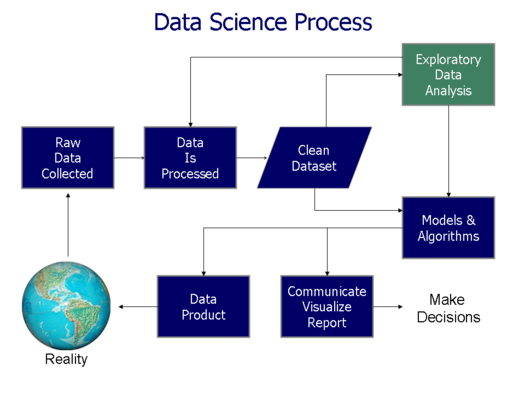
\includegraphics[width=\textwidth]{Data_visualization_process_v1.png}
            % \caption{Data science process flowchart}
        \end{column}
    \end{columns}
    \vspace*{\fill}
\end{frame}

% \subsection{Operational environment}
\begin{frame}
    \frametitle{Operational environment: Maintenance}
    \vspace*{\fill}
    %In the numerous areas in which data analysis shines, 
    We focus on \structure{Maintenance}, where the
    priority is ensuring system reliability and safety during life cycles.
    The basic types are: % of maintenance
    \pause
    \begin{enumerate}
        \item \textbf{Reinforcement} % where equipment is reinforced and hardened to prevent failure
        \item \textbf{Corrective maintenance} % where equipment is repaired or replaced after wear, malfunction or break down
        \item \textbf{Preventive maintenance} % where equipment is checked and serviced in a planned manner; three subtypes:
    \end{enumerate}

    \pause
    \structure{Preventive maintenance} can be further divided into 3 types:
    \pause
    \begin{enumerate}% preventive, predictive, and prescriptive 
        \item[(A)] \acl{ppm} %calendar or usage based
        \item[(B)] \acl{PdM} %based on historical data
        \item[(C)] \acl{cbm} %\textit{maintenance when it is needed}
    \end{enumerate}

    \vspace*{\fill}
\end{frame}

